This chapter will give a general overview on the pieces of technical equipement which we are using and show what the purpose of each one is. In addition, a diagram of the wiring of the components can be found in appendix X. %Wiring.png

\section{Prototype Hardware}

\subsubsection{Motors}
Controlling a quadcopter can be done efficiently by using high-quality motors with fast response, which will ensure more of a stable flight. The motors must also be powerful enough to be able to lift the quadcopter and perform the required aerial movements. 

The motor that we are using is the Turnigy Multistar Brushless Motor seen in Figure \ref{motor}.

\begin{figure}[H]
  \centering
    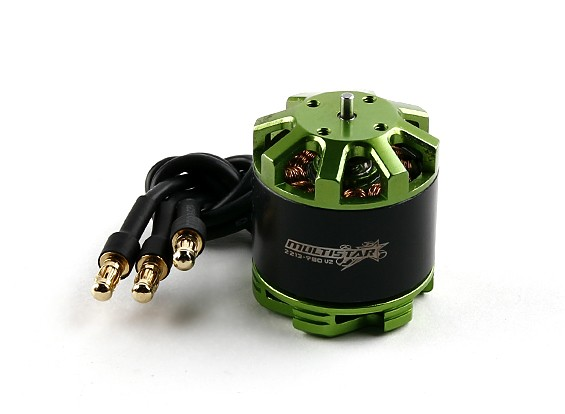
\includegraphics[width=0.5\textwidth]{images/motor.jpg}
	\caption{Turnigy Multistar 2213-980 V2 Brushless Motor}
	\label{motor}
\end{figure}

\subsubsection{Propellers}
The propellers don't have such strict requirements as the motors. They are needed to be light and have a size and lift potential in order for the quadcopter to hover at less than 50\% of the motor capacity. For our quadcopter, we are using plasting 10x4.5'' propellers with light weight - 60g. They have a length of 254 mm and a pitch inclination of 114mm. They can be seen in Figure \ref{propeller}.

\begin{figure}[H]
  \centering
    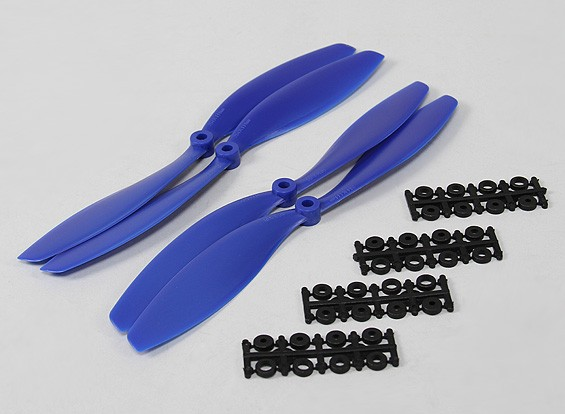
\includegraphics[width=0.5\textwidth]{images/propeller.jpg}
	\caption{Hobbyking Slowfly Propeller 10x4.5}
	\label{propeller}
\end{figure}

\subsubsection{Electric Speed Controller}
Electronic Speed Controller (ESC) is a widely used device in rotorcrafts. The purpose of an ESC is to vary the electric motor's speed. They also come with programmable features, such as braking or selecting appropriate type of battery. We need the ESC to have a fast response, for the same reasons mentioned for the motors in Section \ref{Motors}. The ESC that we are using is the TURNIGY Plush 30A which is shown in Figure \ref{esc}.
 
\begin{figure}[H]
  \centering
    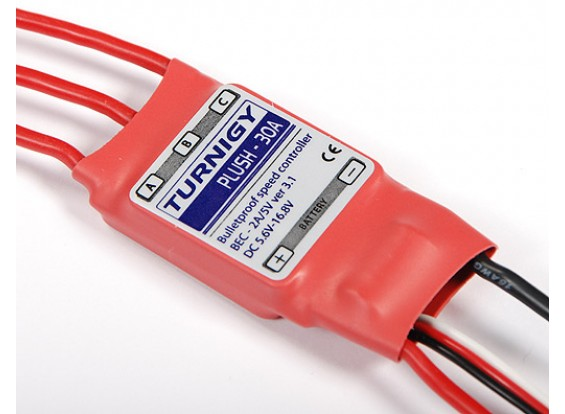
\includegraphics[width=0.5\textwidth]{images/esc.jpg}
	\caption{TURNIGY Plush 30A Speed Controller}
	\label{esc}
\end{figure}

\subsubsection{APM Flight Controller}
ArduPilotMega (APM) is an open source unmanned aerial vehicle (UAV) platform which is able to control autonomous multicopters. It is illustrated in Figure \ref{ardupilot}. The system was improved uses Inertial Measurement Unit (IMU) - a combination of accelerometers, gyroscopes and magnetometers. The "Ardu" part of the project name shows that the programming can be done using Arduino open-source language.

\begin{figure}[H]
  \centering
    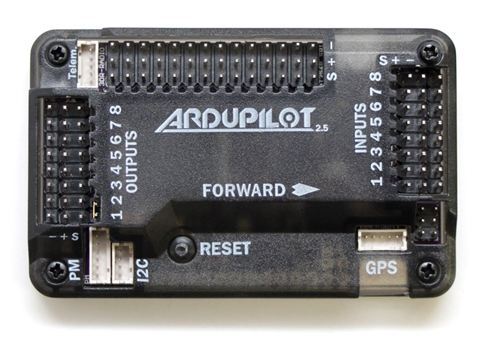
\includegraphics[width=0.5\textwidth]{images/ardupilot.jpg}
	\caption{APM 2.5 board}
	\label{ardupilot}
\end{figure}

\subsubsection{Power Distribution Board}
To reduce the number of connections straight to the battery, we used the a power distribution board made for a previous project. A board like this is an easy solution since it enables us to connect the four ESCs directly to the board and then connect the board to the battery.

\clearpage

\subsubsection{Battery}
To power up our quadcopter, we will use a TURNIGY nano-tech Lipoly battery, which can be seen in Figure \ref{battery}. Higher voltage under load, straighter discharge curves and excellent performance are the factors that make it suitable for our project. 

\begin{figure}[H]
  \centering
    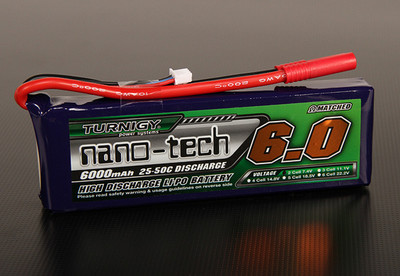
\includegraphics[width=0.5\textwidth]{images/battery.jpg}
	\caption{Turnigy nano-tech 6000mah 3S 25~50C Lipo Pack}
	\label{battery}
\end{figure}

\section{Prototype Measurements}
mass, length, height, moment of inertia

%add quadcopter 'skeleton' and wiring between all this and picture